\documentclass[8pt,aspectratio=169]{beamer}
\usetheme{Madrid}
\usepackage{graphicx}
\usepackage{booktabs}
\usepackage{adjustbox}
\usepackage{multicol}
\usepackage{amsmath}
\usepackage{amssymb}
\usepackage{tikz}
\usepackage{hyperref}
\usepackage{algorithm}
\usepackage{algorithmic}
\usepackage{colortbl}
\usepackage{pgfplots}
\pgfplotsset{compat=1.18}

% TikZ libraries for comics, diagrams, stakeholder maps
\usetikzlibrary{arrows.meta,positioning,shapes.callouts,shapes.geometric,decorations.pathreplacing}

% Color definitions
\definecolor{mlblue}{RGB}{0,102,204}
\definecolor{mlpurple}{RGB}{51,51,178}
\definecolor{mllavender}{RGB}{173,173,224}
\definecolor{mllavender2}{RGB}{193,193,232}
\definecolor{mllavender3}{RGB}{204,204,235}
\definecolor{mllavender4}{RGB}{214,214,239}
\definecolor{mlorange}{RGB}{255, 127, 14}
\definecolor{mlgreen}{RGB}{44, 160, 44}
\definecolor{mlred}{RGB}{214, 39, 40}
\definecolor{mlgray}{RGB}{127, 127, 127}
\definecolor{lightgray}{RGB}{240, 240, 240}
\definecolor{midgray}{RGB}{180, 180, 180}

% NEW COLORS for mini-lecture
\definecolor{dfteal}{RGB}{0,128,128}
\definecolor{dfred}{RGB}{180,30,30}

% Backward compatibility
\colorlet{MLPurple}{mlpurple}
\colorlet{MLBlue}{mlblue}
\colorlet{MLOrange}{mlorange}
\colorlet{MLGreen}{mlgreen}
\colorlet{MLRed}{mlred}
\colorlet{MLLavender}{mllavender}
\colorlet{MLGray}{mlgray}

% Theme colors (exact Madrid settings)
\setbeamercolor{palette primary}{bg=mllavender3,fg=mlpurple}
\setbeamercolor{palette secondary}{bg=mllavender2,fg=mlpurple}
\setbeamercolor{palette tertiary}{bg=mllavender,fg=white}
\setbeamercolor{palette quaternary}{bg=mlpurple,fg=white}
\setbeamercolor{structure}{fg=mlpurple}
\setbeamercolor{section in toc}{fg=mlpurple}
\setbeamercolor{subsection in toc}{fg=mlblue}
\setbeamercolor{title}{fg=mlpurple}
\setbeamercolor{frametitle}{fg=mlpurple,bg=mllavender3}
\setbeamercolor{block title}{bg=mllavender2,fg=mlpurple}
\setbeamercolor{block body}{bg=mllavender4,fg=black}
\setbeamertemplate{navigation symbols}{}
\setbeamertemplate{itemize items}[circle]
\setbeamertemplate{enumerate items}[default]
\setbeamersize{text margin left=5mm,text margin right=5mm}

% Footer
\setbeamertemplate{footline}{
  \leavevmode%
  \hbox{%
    \begin{beamercolorbox}[wd=.333333\paperwidth,ht=2.25ex,dp=1ex,center]{author in head/foot}%
      \usebeamerfont{author in head/foot}Methods and Algorithms
    \end{beamercolorbox}%
    \begin{beamercolorbox}[wd=.333333\paperwidth,ht=2.25ex,dp=1ex,center]{title in head/foot}%
      \usebeamerfont{title in head/foot}MSc Data Science
    \end{beamercolorbox}%
    \begin{beamercolorbox}[wd=.333333\paperwidth,ht=2.25ex,dp=1ex,right]{date in head/foot}%
      \usebeamerfont{date in head/foot}\insertframenumber{} / \inserttotalframenumber\hspace*{2ex}
    \end{beamercolorbox}}%
  \vskip0pt%
}

\newcommand{\bottomnote}[1]{%
\vfill
\vspace{-2mm}
\textcolor{mllavender2}{\rule{\textwidth}{0.4pt}}
\vspace{1mm}
\footnotesize
\textbf{#1}
}

\newenvironment{compactlist}{%
  \begin{itemize}%
    \setlength{\itemsep}{2pt}%
    \setlength{\parskip}{0pt}%
    \setlength{\parsep}{0pt}%
}{%
  \end{itemize}%
}

\newcommand{\highlight}[1]{\textcolor{mlorange}{\textbf{#1}}}
\newcommand{\mathbold}[1]{\boldsymbol{#1}}

\title[t-SNE Mini-Lecture]{t-SNE: Visualizing High-Dimensional Data}
\subtitle{Mini-Lecture: Seeing Hidden Structure in Your Data}
\author{Methods \& Algorithms}
\date{MSc Data Science -- Spring 2026}

\begin{document}

%% ================================================================
%% SLIDE 1: Title Page
%% ================================================================
\begin{frame}[plain]
\titlepage
\end{frame}

%% ================================================================
%% SLIDE 2: WHY -- Opening TikZ Comic
%% ================================================================
\begin{frame}[t]{Why Can't We See 50 Variables at Once?}
\begin{columns}[T]
\column{0.55\textwidth}
\small
\textbf{The Visualization Wall}
\begin{compactlist}
\item You track 1000 stocks with 50 features each (returns, volatility, sector, momentum\ldots)
\item A scatter plot needs 2 axes -- where do the other 48 go?
\item Pairwise plots? That is $\binom{50}{2} = 1225$ scatter plots
\item We need a way to compress 50D into 2D \emph{without losing structure}
\end{compactlist}

\column{0.42\textwidth}
\vspace{2mm}
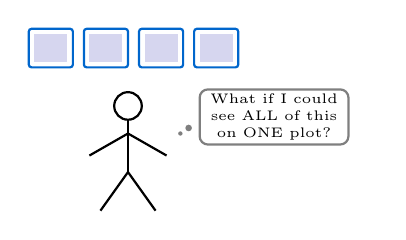
\begin{tikzpicture}[scale=0.7]
  % Analyst stick figure
  \draw[thick] (1.5,3.5) circle (0.25);
  \draw[thick] (1.5,3.25) -- (1.5,2.3);
  \draw[thick] (1.5,3.0) -- (0.8,2.6);
  \draw[thick] (1.5,3.0) -- (2.2,2.6);
  \draw[thick] (1.5,2.3) -- (1.0,1.6);
  \draw[thick] (1.5,2.3) -- (2.0,1.6);
  % Multiple screens
  \foreach \x in {-0.3, 0.7, 1.7, 2.7} {
    \draw[mlblue, thick, rounded corners=1pt] (\x,4.2) rectangle (\x+0.8,4.9);
    \fill[mllavender4] (\x+0.1,4.3) rectangle (\x+0.7,4.8);
  }
  % Thought bubble
  \draw[mlgray, thick, rounded corners=3pt] (2.8,2.8) rectangle (5.5,3.8);
  \node[font=\tiny, text width=2.4cm, align=center] at (4.15,3.3) {What if I could see ALL of this on ONE plot?};
  \fill[mlgray] (2.6,3.1) circle (0.06);
  \fill[mlgray] (2.45,3.0) circle (0.04);
\end{tikzpicture}
\end{columns}

\bottomnote{Human vision is limited to 3D -- dimensionality reduction bridges the gap between data complexity and perception}
\end{frame}

%% ================================================================
%% SLIDE 3: FEEL -- Reflection
%% ================================================================
\begin{frame}[t]{You Have 1000 Stocks and 50 Features}
\begin{columns}[T]
\column{0.95\textwidth}
\small
\textbf{Think About It}
\begin{compactlist}
\item Imagine your data matrix: 1000 rows (stocks) $\times$ 50 columns (features)
\item Each stock lives in a 50-dimensional space -- impossible to visualize directly
\item \highlight{Key intuition}: stocks in the same sector probably cluster together in this 50D space
\item The clusters are \emph{there} -- we just cannot see them
\end{compactlist}

\vspace{3mm}
\begin{block}{The Question}
\scriptsize Is there an algorithm that can project 50D onto 2D while keeping similar stocks close together?
\end{block}

\vspace{2mm}
\scriptsize \textbf{Spoiler}: PCA tries to preserve \emph{global variance}. t-SNE tries to preserve \emph{local neighborhoods}. For discovering clusters, neighborhoods matter more.
\end{columns}

\bottomnote{Dimensionality reduction is not about throwing away data -- it is about revealing hidden structure}
\end{frame}

%% ================================================================
%% SLIDE 4: WHAT -- Plain English Definition
%% ================================================================
\begin{frame}[t]{What IS t-SNE?}
\begin{columns}[T]
\column{0.55\textwidth}
\small
\textbf{t-SNE in Plain English}

An algorithm that squeezes high-dimensional data into 2D while preserving which points are \highlight{neighbors}.

\vspace{3mm}
\textbf{Key Terms}
\begin{compactlist}
\item \highlight{Embedding}: the 2D output -- each point gets an $(x,y)$ coordinate
\item \highlight{Perplexity}: how many neighbors each point ``pays attention to'' (typically 5--50)
\item \highlight{Neighborhood}: points that are close in the original 50D space
\end{compactlist}

\begin{block}{Core Idea}
\scriptsize If two stocks are similar in 50D, they should land near each other in 2D. If they are different, they should be far apart.
\end{block}

\column{0.42\textwidth}
\vspace{2mm}
\footnotesize
\fcolorbox{mlpurple}{mllavender4}{\parbox{0.85\columnwidth}{%
\textbf{t-SNE stands for:}

\vspace{2mm}
\textbf{t}-distributed

\textbf{S}tochastic

\textbf{N}eighbor

\textbf{E}mbedding

\vspace{2mm}
van der Maaten \& Hinton (2008)
}}
\end{columns}

\bottomnote{t-SNE is for \emph{visualization only} -- do not use the 2D coordinates as features for a downstream model}
\end{frame}

%% ================================================================
%% SLIDE 5: CASE -- Chart: t-SNE Perplexity 30
%% ================================================================
\begin{frame}[t]{How Does t-SNE Reveal Hidden Structure?}
\begin{columns}[T]
\column{0.55\textwidth}

\includegraphics[width=\textwidth]{04b_tsne_perplexity_30/chart.pdf}

\column{0.42\textwidth}
\small
\textbf{What You See}
\begin{compactlist}
\item Each dot is a data point (e.g.\ a stock described by 50 features)
\item Colors represent true groups (sectors, regimes)
\item t-SNE places similar points close together in 2D
\item Clusters emerge that were invisible in raw data tables
\end{compactlist}

\begin{block}{Finance Interpretation}
\scriptsize Tech stocks cluster together, banks cluster together, energy stocks cluster together -- because their 50-feature profiles are similar.
\end{block}
\end{columns}

\bottomnote{Perplexity=30 (sklearn default) balances local and global structure -- always a good starting point}
\end{frame}

%% ================================================================
%% SLIDE 6: HOW -- Chart: Cluster Projection
%% ================================================================
\begin{frame}[t]{How Does t-SNE Preserve Neighborhoods?}
\begin{columns}[T]
\column{0.55\textwidth}

\includegraphics[width=\textwidth]{06c_tsne_cluster_projection/chart.pdf}

\column{0.42\textwidth}
\small
\textbf{The Neighborhood Rule}
\begin{compactlist}
\item Points close in high-D stay close in 2D
\item Points far apart in high-D get pushed further apart
\item The algorithm minimizes the mismatch between high-D and low-D neighborhoods
\item Result: clusters that overlap in PCA become separated in t-SNE
\end{compactlist}

\begin{block}{Key Difference from PCA}
\scriptsize PCA preserves \emph{directions of maximum spread}. t-SNE preserves \emph{who is near whom}.
\end{block}
\end{columns}

\bottomnote{t-SNE uses a Student-t distribution in low-D to prevent the ``crowding problem'' -- moderate distances get room to spread}
\end{frame}

%% ================================================================
%% SLIDE 7: RISK -- TikZ Comic: Parameter Sensitivity
%% ================================================================
\begin{frame}[t]{What Can Go Wrong with t-SNE?}
\begin{columns}[T]
\column{0.55\textwidth}
\small
\textbf{Parameter Sensitivity}
\begin{compactlist}
\item Different perplexity values produce different cluster layouts
\item Different random seeds produce different orientations
\item Cluster \emph{sizes} in 2D are meaningless
\item Distances \emph{between} clusters are meaningless
\end{compactlist}

\begin{block}{Golden Rule}
\scriptsize Always run t-SNE with at least 3 different perplexity values. If a pattern disappears when you change perplexity, it is an artifact.
\end{block}

\column{0.42\textwidth}
\vspace{2mm}
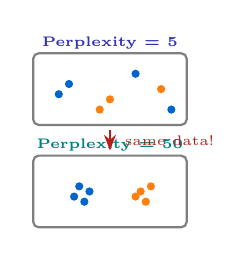
\begin{tikzpicture}[scale=0.65]
  % Map 1: perplexity=5
  \node[font=\tiny\bfseries, mlpurple] at (1.5,4.8) {Perplexity = 5};
  \draw[mlgray, thick, rounded corners=2pt] (0,3.2) rectangle (3,4.6);
  % Many small fragments
  \fill[mlblue] (0.5,3.8) circle (0.08);
  \fill[mlblue] (0.7,4.0) circle (0.08);
  \fill[mlorange] (1.3,3.5) circle (0.08);
  \fill[mlorange] (1.5,3.7) circle (0.08);
  \fill[mlblue] (2.0,4.2) circle (0.08);
  \fill[mlorange] (2.5,3.9) circle (0.08);
  \fill[mlblue] (2.7,3.5) circle (0.08);
  % Map 2: perplexity=50
  \node[font=\tiny\bfseries, dfteal] at (1.5,2.8) {Perplexity = 50};
  \draw[mlgray, thick, rounded corners=2pt] (0,1.2) rectangle (3,2.6);
  % Two clean clusters
  \fill[mlblue] (0.8,1.8) circle (0.08);
  \fill[mlblue] (0.9,2.0) circle (0.08);
  \fill[mlblue] (1.0,1.7) circle (0.08);
  \fill[mlblue] (1.1,1.9) circle (0.08);
  \fill[mlorange] (2.1,1.9) circle (0.08);
  \fill[mlorange] (2.2,1.7) circle (0.08);
  \fill[mlorange] (2.3,2.0) circle (0.08);
  \fill[mlorange] (2.0,1.8) circle (0.08);
  % Arrow
  \draw[-{Stealth[length=2mm]}, dfred, thick] (1.5,3.1) -- (1.5,2.7);
  \node[font=\tiny, dfred, right] at (1.6,2.9) {same data!};
\end{tikzpicture}
\end{columns}

\bottomnote{Wattenberg et al.\ (2016) ``How to Use t-SNE Effectively'' -- required reading before interpreting t-SNE plots}
\end{frame}

%% ================================================================
%% SLIDE 8: WHERE -- Finance Applications
%% ================================================================
\begin{frame}[t]{Where Do Quants Use t-SNE?}
\begin{columns}[T]
\column{0.95\textwidth}
\small
\textbf{Four Key Applications in Finance}

\vspace{2mm}
\footnotesize
\begin{tabular}{@{}l p{9.5cm}@{}}
\toprule
\textbf{Application} & \textbf{How It Works} \\
\midrule
\rowcolor{mllavender4}
\highlight{Market Regime Detection} & Project daily return vectors of 50 stocks into 2D. Color by date. Clusters = regimes (bull, bear, crisis). \\
Portfolio Visualization & Map 500 stocks by their 50 risk factors. See which stocks group together without sector labels. \\
\rowcolor{mllavender4}
Anomaly Detection & Points far from any cluster in the t-SNE map are potential outliers -- flash crashes, rogue trades. \\
Customer Segmentation & Visualize banking customers by 30+ behavioral features. Discover natural groups for product targeting. \\
\bottomrule
\end{tabular}
\end{columns}

\bottomnote{t-SNE is an exploration tool -- it generates hypotheses about structure, which you then test with statistical methods}
\end{frame}

%% ================================================================
%% SLIDE 9: SO WHAT -- t-SNE vs PCA
%% ================================================================
\begin{frame}[t]{When Should You Use t-SNE vs PCA?}
\begin{columns}[T]
\column{0.95\textwidth}
\small

\vspace{1mm}
\footnotesize
\begin{tabular}{@{}l c c@{}}
\toprule
\textbf{Use Case} & \textbf{\textcolor{dfteal}{PCA}} & \textbf{\textcolor{mlpurple}{t-SNE}} \\
\midrule
\rowcolor{mllavender4}
Need new coordinate system & \checkmark & \\
Preprocessing for ML model & \checkmark & \\
\rowcolor{mllavender4}
Interpretable axes (loadings) & \checkmark & \\
Discovering hidden clusters & & \checkmark \\
\rowcolor{mllavender4}
Exploring non-linear structure & & \checkmark \\
Presenting to non-technical audience & & \checkmark \\
\rowcolor{mllavender4}
Speed matters ($n > 10{,}000$) & \checkmark & \\
Projecting new data points & \checkmark & \\
\bottomrule
\end{tabular}

\vspace{3mm}
\begin{block}{Best Practice}
\scriptsize Run PCA first to reduce to 30--50 dimensions, then apply t-SNE on the PCA output. This is faster, more stable, and removes noise.
\end{block}
\end{columns}

\bottomnote{PCA is a tool (transforms data for modeling). t-SNE is a lens (shows you what the data looks like). Use both.}
\end{frame}

%% ================================================================
%% SLIDE 10: ACT -- Summary + Closing TikZ
%% ================================================================
\begin{frame}[t]{Summary: t-SNE in 4 Takeaways}
\begin{columns}[T]
\column{0.55\textwidth}
\small
\begin{enumerate}
\setlength{\itemsep}{5pt}
\item \highlight{t-SNE preserves neighborhoods}: similar points in high-D land near each other in 2D
\item \highlight{Perplexity controls the view}: low = local detail, high = global structure. Always try 3+ values.
\item \highlight{Do not over-interpret}: cluster sizes, inter-cluster distances, and axis orientation are meaningless
\item \highlight{Finance use}: regime detection, anomaly spotting, and portfolio visualization
\end{enumerate}

\begin{block}{Next Steps}
\scriptsize Explore the deep dive for KL divergence derivation, the crowding problem, and UMAP comparison.
\end{block}

\column{0.42\textwidth}
\vspace{4mm}
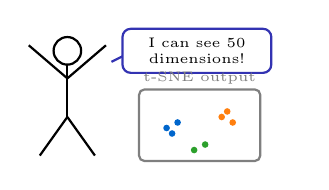
\begin{tikzpicture}[scale=0.7]
  % Stick figure celebrating
  \draw[thick] (1.5,3.2) circle (0.25);
  \draw[thick] (1.5,2.95) -- (1.5,2.0);
  \draw[thick] (1.5,2.7) -- (0.8,3.3);
  \draw[thick] (1.5,2.7) -- (2.2,3.3);
  \draw[thick] (1.5,2.0) -- (1.0,1.3);
  \draw[thick] (1.5,2.0) -- (2.0,1.3);
  % Speech bubble
  \draw[mlpurple, thick, rounded corners=3pt] (2.5,2.8) rectangle (5.2,3.6);
  \node[font=\tiny, text width=2.4cm, align=center] at (3.85,3.2) {I can see 50 dimensions!};
  \draw[mlpurple, thick] (2.5,3.1) -- (2.3,3.0);
  % Small t-SNE plot
  \draw[mlgray, thick, rounded corners=2pt] (2.8,1.2) rectangle (5.0,2.5);
  \fill[mlblue] (3.3,1.8) circle (0.06);
  \fill[mlblue] (3.5,1.9) circle (0.06);
  \fill[mlblue] (3.4,1.7) circle (0.06);
  \fill[mlorange] (4.3,2.0) circle (0.06);
  \fill[mlorange] (4.5,1.9) circle (0.06);
  \fill[mlorange] (4.4,2.1) circle (0.06);
  \fill[mlgreen] (3.8,1.4) circle (0.06);
  \fill[mlgreen] (4.0,1.5) circle (0.06);
  \node[font=\tiny, mlgray] at (3.9,2.7) {t-SNE output};
\end{tikzpicture}
\end{columns}

\bottomnote{t-SNE is for exploration, not measurement. Use it to generate hypotheses, then test them with rigorous statistics.}
\end{frame}

\end{document}
